\documentclass[a4paper,landscape,12pt]{extarticle}
\usepackage[left=0.5in,right=0.5in,top=0.4in,bottom=0.55in]{geometry}

\usepackage{graphicx}
\usepackage[normalem]{ulem}
\usepackage{multicol}
\usepackage{array}
\usepackage{caption}
\usepackage{fancyhdr}
\usepackage{lastpage}
\usepackage{amsmath,amssymb}
\usepackage{booktabs}
\usepackage{listings}
\usepackage{xcolor}
\usepackage{hyperref}
\usepackage{circuitikz}

% ---------- Listings (code blocks) ----------
\lstset{
  language=Python,
  basicstyle=\ttfamily\Large,
  keywordstyle=\color{blue}\bfseries,
  commentstyle=\color{gray},
  stringstyle=\color{teal},
  numbers=left,
  numberstyle=\Large\color{gray},
  frame=single,
  breaklines=true,
  breakatwhitespace=true,
  columns=fullflexible,
  keepspaces=true,
  showstringspaces=false
}

\author{Jacky Li}

% Page style with slide numbers
\pagestyle{fancy}
\fancyhf{}
\renewcommand{\headrulewidth}{0pt}
\fancyfoot[R]{\Large\thepage\ / \pageref{LastPage}}

% Header (expects cpp_logo.png in same folder)
\newcommand{\slideheader}[2]{%
\noindent

\includegraphics[height=0.5in]{cpp_logo.png}%
\hspace{0.3in}%
{\Large \uline{#1 \hfill #2}}%
\par\vspace{0.4in}
}

\begin{document}
\begin{huge}

%%%%%%%%%%%%%%%%%%%%%%%%%%%%%%%%%%%%%%%%%%%%%%%%%%%%%%%%%%%%
% SLIDE 1 - Title Slide
%%%%%%%%%%%%%%%%%%%%%%%%%%%%%%%%%%%%%%%%%%%%%%%%%%%%%%%%%%%%
\slideheader{ECE 5110 Numerical Modeling}{Jacky Li}

\vspace{1.0in}
\begin{center}
{\Huge \textbf{Newton's Method Seminar}}

\vspace{0.35in}
{\LARGE Unit 1: Solution of Equations in One Variable}\\
\vspace{0.15in}
{\LARGE \textbf{Diode Circuit Operating Point Analysis}}

\vspace{0.35in}
{\Large February 09, 2025}
\end{center}

\newpage

%%%%%%%%%%%%%%%%%%%%%%%%%%%%%%%%%%%%%%%%%%%%%%%%%%%%%%%%%%%%
% SLIDE 2 - Outline
%%%%%%%%%%%%%%%%%%%%%%%%%%%%%%%%%%%%%%%%%%%%%%%%%%%%%%%%%%%%
\slideheader{Outline}{Newton's Method}

\leftskip 0.7in \rightskip 0.7in
\vspace{0.2in}

\begin{itemize}
  \item Motivation: Root finding in engineering
  \item Problem: Series resistor--diode DC operating point
  \item Formulation: Residual function $f(V_d)=0$
  \item Newton's method algorithm and convergence
  \item Implementation (Python): \texttt{solve\_newton}
  \item Results: operating point and convergence plots
  \item Comparison: Newton vs. bisection
  \item Discussion and conclusion
\end{itemize}

\leftskip 0in \rightskip 0in
\newpage

%%%%%%%%%%%%%%%%%%%%%%%%%%%%%%%%%%%%%%%%%%%%%%%%%%%%%%%%%%%%
% SLIDE 3 - Root finding overview
%%%%%%%%%%%%%%%%%%%%%%%%%%%%%%%%%%%%%%%%%%%%%%%%%%%%%%%%%%%%
\slideheader{Root-Finding Methods}{Newton's Method}

\leftskip 0.7in \rightskip 0.7in
\vspace{0.15in}

\begin{multicols}{2}
\textbf{Bisection Method}
\begin{itemize}
  \item Guaranteed convergence if sign change on $[a,b]$
  \item No derivative required
  \item Linear convergence (slow)
  \item Often used as a reliable fallback
\end{itemize}

\columnbreak

\textbf{Newton's Method}
\begin{itemize}
  \item Quadratic convergence near a simple root
  \item Requires derivative $f'(x)$
  \item Sensitive to initial guess
  \item Standard in circuit simulation (Newton--Raphson)
\end{itemize}
\end{multicols}

\vspace{0.25in}
\textbf{Goal:} Apply Newton’s method to a practical EE nonlinear equation (diode operating point).

\leftskip 0in \rightskip 0in
\newpage

%%%%%%%%%%%%%%%%%%%%%%%%%%%%%%%%%%%%%%%%%%%%%%%%%%%%%%%%%%%%
% SLIDE 4 - Problem formulation (with circuit diagram)
%%%%%%%%%%%%%%%%%%%%%%%%%%%%%%%%%%%%%%%%%%%%%%%%%%%%%%%%%%%%
\slideheader{Problem: Diode Circuit Operating Point}{Newton's Method}

\leftskip 0.7in \rightskip 0.7in
\vspace{0.05in}

\begin{multicols}{2}

% LEFT
KVL:
\[
V_s = IR + V_d
\]

Shockley:
\[
I = I_s (e^{V_d/(nV_T)} - 1)
\]

Residual:
\[
f(V_d)= I_s\left(e^{\,V_d/(nV_T)} - 1\right) - \frac{V_s - V_d}{R} = 0
\]

\columnbreak

% RIGHT
\begin{center}
\begin{circuitikz}[scale=1.3, transform shape]
    \draw (0,0) to[V, v=$V_s$, invert] (0,3)
          to[R, l=$R$, i=$I$] (4,3)
          to[D, l=$D$, v=$V_d$] (4,0)
          -- (0,0);
    \draw (0,0) node[ground]{};
\end{circuitikz}

\vspace{0.1in}
Series resistor–diode circuit.
\end{center}
\end{multicols}


\leftskip 0in \rightskip 0in
\newpage


%%%%%%%%%%%%%%%%%%%%%%%%%%%%%%%%%%%%%%%%%%%%%%%%%%%%%%%%%%%%
% SLIDE 5 - Newton method algorithm
%%%%%%%%%%%%%%%%%%%%%%%%%%%%%%%%%%%%%%%%%%%%%%%%%%%%%%%%%%%%
\slideheader{Newton's Method Algorithm}{Newton's Method}

\leftskip 0.7in \rightskip 0.7in
\vspace{0.1in}

\textbf{Iteration:}
\[
x_{k+1} = x_k - \frac{f(x_k)}{f'(x_k)}
\]

\textbf{Stopping criterion:}
\[
|f(x_k)| < \varepsilon
\]

\textbf{Quadratic convergence (near a simple root):}
If $x^*$ is a simple root and $f'(x^*)\neq 0$, then the error approximately satisfies
\[
e_{k+1} \approx C\,e_k^2
\quad\Rightarrow\quad \text{error squares each iteration.}
\]

\vspace{0.15in}
\textbf{Why it works well here:}
\begin{itemize}
  \item Smooth monotone function for $V_d>0$
  \item Easy-to-compute derivative
  \item Reasonable initial guess (e.g., $V_d^{(0)}=0.5$ V)
\end{itemize}

\leftskip 0in \rightskip 0in
\newpage

%%%%%%%%%%%%%%%%%%%%%%%%%%%%%%%%%%%%%%%%%%%%%%%%%%%%%%%%%%%%
% SLIDE 6 - Implementation (code)
%%%%%%%%%%%%%%%%%%%%%%%%%%%%%%%%%%%%%%%%%%%%%%%%%%%%%%%%%%%%
\slideheader{Implementation: Python Solver (No Plot Code)}{Jacky Li}

\leftskip 0.7in \rightskip 0.7in
\vspace{0.05in}

\begin{lstlisting}
def solve_newton(self, f, df, x0, precision=1e-6, max_steps=100):
    x = x0
    history = []
    for step in range(1, max_steps + 1):
        fx  = f(x)
        dfx = df(x)
        history.append((step, x, fx))

        if abs(fx) < precision:
            return x, 0, history        # converged
        if abs(dfx) < 1e-15:
            return x, -2, history       # derivative too small

        x = x - fx / dfx

    return x, -1, history               # did not converge
\end{lstlisting}

\vspace{0.15in}
\textbf{Note:} Plotting is only done in the unit test file (e.g., \texttt{unit01\_newton.py}).

\leftskip 0in \rightskip 0in
\newpage

%%%%%%%%%%%%%%%%%%%%%%%%%%%%%%%%%%%%%%%%%%%%%%%%%%%%%%%%%%%%
% SLIDE 7 - Results: operating point + combined plot
%%%%%%%%%%%%%%%%%%%%%%%%%%%%%%%%%%%%%%%%%%%%%%%%%%%%%%%%%%%%
\slideheader{Results: Operating Point and Convergence}{Newton's Method}

\leftskip 0.7in \rightskip 0.7in
\vspace{0.05in}

\begin{multicols}{2}
\textbf{Operating point (Newton):}
\[
V_d \approx 0.8587\ \text{V}
\qquad
I \approx 4.141\ \text{mA}
\]
Converges in about \textbf{8 iterations} (quadratic drop in $|f(V_d)|$).

\columnbreak

\begin{center}
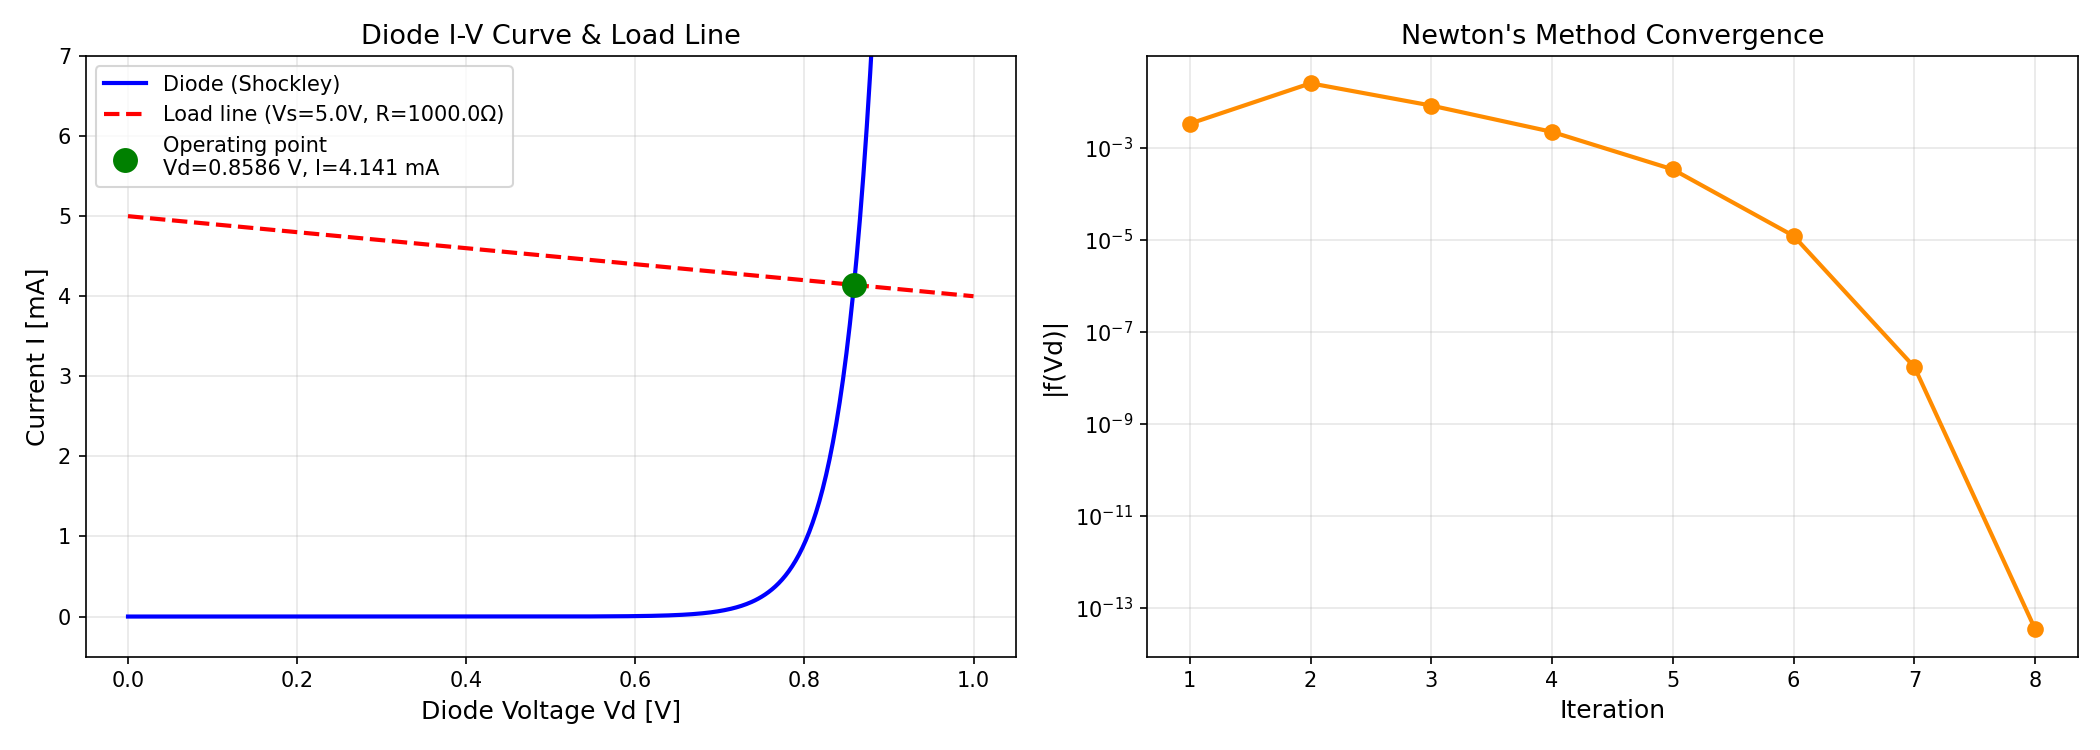
\includegraphics[width=0.92\linewidth]{newton_diode_results.png}
\end{center}
\end{multicols}

\leftskip 0in \rightskip 0in
\newpage

%%%%%%%%%%%%%%%%%%%%%%%%%%%%%%%%%%%%%%%%%%%%%%%%%%%%%%%%%%%%
% SLIDE 8 - Comparison: Newton vs Bisection
%%%%%%%%%%%%%%%%%%%%%%%%%%%%%%%%%%%%%%%%%%%%%%%%%%%%%%%%%%%%
\slideheader{Convergence Comparison: Newton vs Bisection}{Newton's Method}

\leftskip 0.7in \rightskip 0.7in
\vspace{0.05in}

\begin{center}
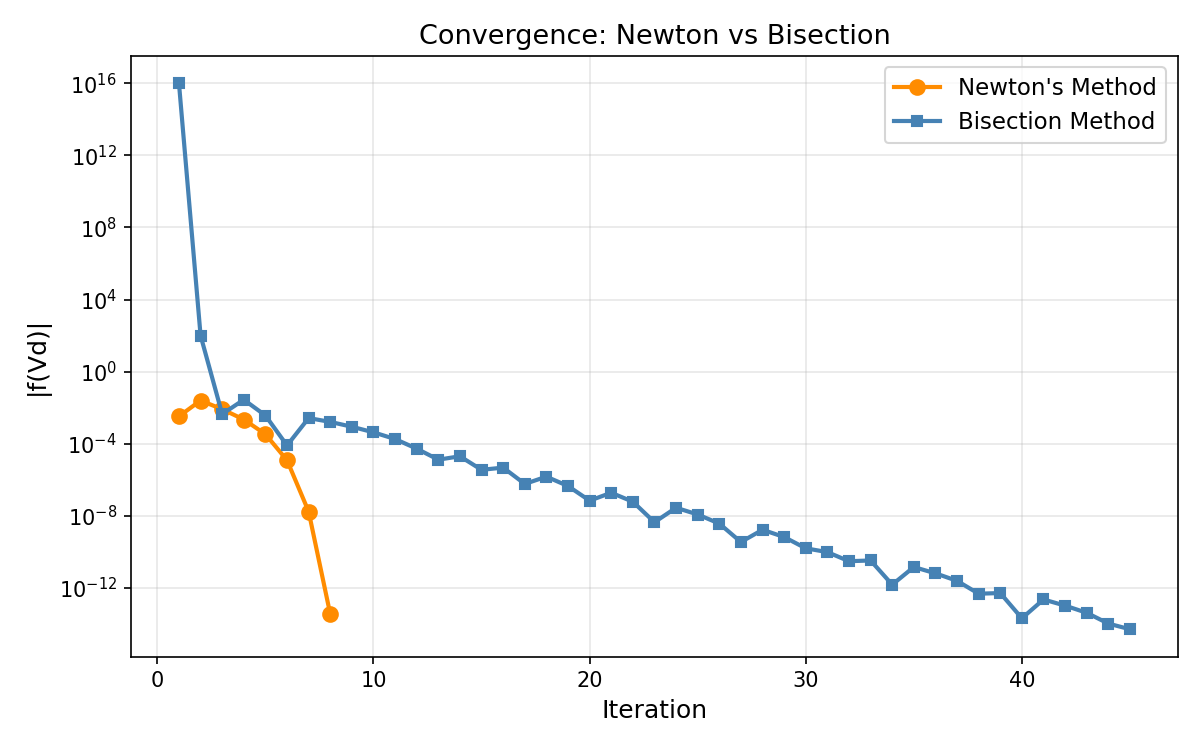
\includegraphics[width=0.62\textwidth]{newton_vs_bisection.png}
\end{center}

\vspace{0.15in}
\begin{itemize}
  \item \textbf{Newton:} reaches $\sim 10^{-10}$ in $\sim 8$ iterations (quadratic convergence)
  \item \textbf{Bisection:} needs $\sim 50$ iterations for similar tolerance (linear convergence)
\end{itemize}

\leftskip 0in \rightskip 0in
\newpage

%%%%%%%%%%%%%%%%%%%%%%%%%%%%%%%%%%%%%%%%%%%%%%%%%%%%%%%%%%%%
% SLIDE 9 - Discussion + Conclusion
%%%%%%%%%%%%%%%%%%%%%%%%%%%%%%%%%%%%%%%%%%%%%%%%%%%%%%%%%%%%
\slideheader{Discussion and Conclusion}{Jacky Li}

\leftskip 0.7in \rightskip 0.7in
\vspace{0.05in}

\begin{multicols}{2}
\textbf{Advantages of Newton's Method}
\begin{itemize}
  \item Very fast (quadratic) convergence
  \item Few iterations for high accuracy
  \item No bracketing interval required
  \item Used in SPICE-style nonlinear circuit solvers
\end{itemize}

\textbf{Disadvantages}
\begin{itemize}
  \item Requires $f'(x)$
  \item Sensitive to initial guess
  \item No universal convergence guarantee
\end{itemize}

\columnbreak

\textbf{Conclusion}
\begin{itemize}
  \item Formulated diode DC operating point as $f(V_d)=0$
  \item Newton converged to
  \[
  V_d \approx 0.859\ \text{V},\quad I \approx 4.14\ \text{mA}
  \]
  \item Demonstrated clear quadratic vs. linear convergence (bisection)
  \item Best when derivative and a reasonable initial guess are available
\end{itemize}
\end{multicols}

\leftskip 0in \rightskip 0in

\end{huge}
\end{document}
